\documentclass[
	11pt,
	BCOR=5mm,
	DIV=12,
	headinclude=on,
	footinclude=off,
	footheight = 23.39284pt,
	parskip=half,
	bibliography=totoc,
	listof=entryprefix,
	toc=listof,
	numbers=noenddot,
	plainfootsepline]{scrreprt}

%	Konfigurationsdatei einziehen

% !TEX root =  master.tex

%		LANGUAGE SETTINGS AND FONT ENCODING 
%
\usepackage[ngerman]{babel} 	% German language
\usepackage[utf8]{inputenc}
\usepackage[german=quotes]{csquotes} 	% correct quotes using \enquote{}
\usepackage[T1]{fontenc}
\usepackage[onehalfspacing]{setspace}
\usepackage[left=1.8cm,right=2.7cm,top=4cm,bottom=3cm]{geometry}
\usepackage{setspace}
\singlespacing
\usepackage{glossaries}
% \usepackage{pdfpages}
\usepackage{array}
\usepackage{scrhack}
%\usepackage[english]{babel}   % For english language
%\usepackage{csquotes} 	% Richtiges Setzen der Anführungszeichen mit \enquote{}

% 		HYPERREF
%
\usepackage[hidelinks]{hyperref} % Keine roten Markierungen bei Links

% Eigene Befehle zum Setzen von wichtigen Angaben. Ausserdem werden die PDF-Informationen richtig gesetzt.
\newcommand{\TitelDerArbeit}[1]{\def\DerTitelDerArbeit{#1}\hypersetup{pdftitle={#1}}}
\newcommand{\TitelDerArbeitEnglisch}[1]{\def\DerTitelDerArbeitEnglisch{#1}}
\newcommand{\AutorDerArbeit}[1]{\def\DerAutorDerArbeit{#1}\hypersetup{pdfauthor={#1}}}
\newcommand{\Matrikelnummer}[1]{\def\DieMatrikelnummer{#1}}
\newcommand{\Firma}[1]{\def\DerNameDerFirma{#1}}
\newcommand{\Kurs}[1]{\def\DieKursbezeichnung{#1}}


% Correct superscripts 
\usepackage{fnpct}




%		CALCULATIONS
%
\usepackage{calc} % Used for extra space below footsepline



%		BIBLIOGRAPHY SETTINGS
%

% Uncomment the next three lines for author-year-style with footnotes (Chicago)
\usepackage[backend=biber, autocite=footnote, style=authoryear, dashed=false]{biblatex} 	%Use Author-Year-Cites with footnotes
%\AdaptNoteOpt\footcite\multfootcite   %will add  separators if footcite is called multiple consecutive times 
%\AdaptNoteOpt\autocite\multautocite % will add  separators if autocite is called multiple consecutive times

% Uncomment the next line for IEEE-style 
% \usepackage[backend=biber, autocite=inline, style=ieee]{biblatex} 	% Use IEEE-Style (e.g. [1])

% Uncomment the next line for alphabetic style 
% \usepackage[backend=biber, autocite=inline, style=alphabetic]{biblatex} 	% Use alphabetic style (e.g. [TGK12])

% Uncomment the next two lines vor Harvard-Style 
%\usepackage[backend=biber, style=apa]{biblatex} 	
%\DeclareLanguageMapping{german}{german-apa}


\DefineBibliographyStrings{ngerman}{  %Change u.a. to et al. (german only!)
	andothers = {{et\,al\adddot}},
}

%%% Uncomment the following lines to support hard URL breaks in bibliography 
%\apptocmd{\UrlBreaks}{\do\f\do\m}{}{}
%\setcounter{biburllcpenalty}{9000}% Kleinbuchstaben
%\setcounter{biburlucpenalty}{9000}% Großbuchstaben


\setlength{\bibparsep}{\parskip}		%add some space between biblatex entries in the bibliography
\addbibresource{bibliography.bib}	%Add file bibliography.bib as biblatex resource


%		FOOTNOTES 
%
% Count footnotes over chapters
\usepackage{chngcntr}
\counterwithout{footnote}{chapter}

%	ACRONYMS
%%%
%%% WICHTIG: Installieren Sie das neueste Acronyms-Paket!!!
%%%
\makeatletter
\usepackage[printonlyused]{acronym}
\@ifpackagelater{acronym}{2015/03/20}
  {%
    \renewcommand*{\aclabelfont}[1]{\textbf{\textsf{\acsfont{#1}}}}
  }%
  {%
  }%
\makeatother

%		LISTINGS
\usepackage{listings}	%Format Listings properly
\renewcommand{\lstlistingname}{Quelltext} 
\renewcommand{\lstlistlistingname}{Quelltextverzeichnis}
\lstset{numbers=left,
	numberstyle=\tiny,
	captionpos=b,
	basicstyle=\ttfamily\small}


%		EXTRA PACKAGES
\usepackage{lipsum}    %Blindtext
\usepackage{graphicx} % use various graphics formats
\usepackage[german]{varioref} 	% nicer references \vref
\usepackage[center]{caption}	%better Captions
\usepackage{booktabs} %nicer Tabs
\usepackage{array}
\usepackage{tabularx}
\usepackage{multirow}
\usepackage{paralist}
\usepackage{ragged2e}
\usepackage{tabu}

%		ALGORITHMS
\usepackage{algorithm}
\usepackage{algpseudocode}
\renewcommand{\listalgorithmname}{Algorithmenverzeichnis }
\floatname{algorithm}{Algorithmus}


%		FONT SELECTION: Entweder Latin Modern oder Times / Helvetica
\usepackage{lmodern} %Latin modern font
%\usepackage{mathptmx}  %Helvetica / Times New Roman fonts (2 lines)
%\usepackage[scaled=.92]{helvet} %Helvetica / Times New Roman fonts (2 lines)

%		PAGE HEADER / FOOTER
%	    Warning: There are some redefinitions throughout the master.tex-file!  DON'T CHANGE THESE REDEFINITIONS!
\RequirePackage[automark,headsepline,footsepline]{scrlayer-scrpage}
\pagestyle{scrheadings}
\renewcommand*{\pnumfont}{\upshape\sffamily}
\renewcommand*{\headfont}{\upshape\sffamily}
\renewcommand*{\footfont}{\upshape\sffamily}
\renewcommand{\chaptermarkformat}{}
\RedeclareSectionCommand[beforeskip=0pt]{chapter}
\clearscrheadfoot

\ifoot[\rule{0pt}{\ht\strutbox+\dp\strutbox}DHBW Mannheim]{\rule{0pt}{\ht\strutbox+\dp\strutbox}DHBW Mannheim}
\ofoot[\rule{0pt}{\ht\strutbox+\dp\strutbox}\pagemark]{\rule{0pt}{\ht\strutbox+\dp\strutbox}\pagemark}

\ohead{\headmark}

%Java Syntax highlighting
\usepackage{listings}
\usepackage{color}

\definecolor{dkgreen}{rgb}{0,0.6,0}
\definecolor{gray}{rgb}{0.5,0.5,0.5}
\definecolor{mauve}{rgb}{0.58,0,0.82}

\lstset{frame=tb,
  language=Java,
  aboveskip=3mm,
  belowskip=3mm,
  showstringspaces=false,
  columns=flexible,
  basicstyle={\small\ttfamily},
  numbers=none,
  numberstyle=\tiny\color{gray},
  keywordstyle=\color{blue},
  commentstyle=\color{dkgreen},
  stringstyle=\color{mauve},
  breaklines=true,
  breakatwhitespace=true,
  tabsize=3
}

\begin{document}

%% BITTE GEBEN SIE HIER WICHTIGE INFORMATIONEN DER ARBEIT AN!
%% DIESE INFORMATIONEN MÜSSEN GESETZT SEIN, UM TITELBLATT, ABSTRACT UND
%% EIGENSTÄNDIGKEITSERKLÄRUNG AUTOMATISCH ANZUPASSEN!
\TitelDerArbeit{Implementierung vom Minimax Algorithmus und Tic-Tac-Toe in Java}
\TitelDerArbeitEnglisch{Implementation of the Minimax-Algorithm and Tic-Tac-Toe in Java}
\AutorDerArbeit{Fabio Jungmann \& Florian Gölz }
\Matrikelnummer{7527342, 9223147 }
\Kurs{TINF18AI2}

% !TEX root =  master.tex
\begin{titlepage}
\begin{minipage}{\textwidth}
		\vspace{-2cm}
		\noindent \hfill   
\includegraphics{img/logo.jpg}
\end{minipage}
\vspace{3.2em}
\sffamily
\begin{center}
	\textsf{\textbf{HAUSARBEIT}}\\[1cm]
    \textsf{\textbf{\large{}\DerTitelDerArbeit}} \\[1cm]
	\textsf{im Studiengang}\\[3mm]
	\textsf{Angewandte Informatik} 
	\textsf{an der Dualen Hochschule Baden-Württemberg Mannheim} \\[0.7cm]
	\textsf{von}\\[5mm]
	\textsf{\DerAutorDerArbeit} \\[0.6cm]
	\textsf{11.06.2021} \\[0.8cm]
\vfill


\begin{minipage}{\textwidth}

\begin{tabbing}
	Wissenschaftlicher Betreuer: \hspace{0.6cm}\=\kill
	Matrikelnummer, Kurs \>\DieMatrikelnummer \DieKursbezeichnung \\[3mm]
	Ausbildungsfirma \>Detect Value AG, Roche Diagnostics GmbH \\[3mm] 
	Dozent \> Prof. Dr. Karl Stroetmann \\[3mm]
\end{tabbing}
\end{minipage}

\end{center}

\end{titlepage}

\pagenumbering{Roman} % Römische Seitennummerierung
\normalfont

%	Ehrenwörtliche Erklärung
% Wird die folgende Zeile auskommentiert, erscheint die ehrenwörtliche
% Erklärung im Inhaltsverzeichnis.

% \addcontentsline{toc}{chapter}{Ehrenwörtliche Erklärung}
% !TEX root =  master.tex
\clearpage
\chapter*{Ehrenwörtliche Erklärung}

Wir versichern hiermit, dass wir die vorliegende Arbeit
 mit dem Thema \newline\\[2mm] \textbf{\textit{\DerTitelDerArbeit}} \newline\\[2mm] selbstständig verfasst und keine anderen als die angegebenen Quellen und
Hilfsmittel verwendet haben.

\vspace{3cm}
Ort, Datum \hfill \DerAutorDerArbeit


% Sperrvermerk
%\input{sperrvermerk.tex}

%	Anmerkung zur Verwendung geschlechterspezifischer Bezeichnungen (Inklusionsverweis)
% !TEX root =  master.tex
\chapter*{Anmerkung}

Aus Gründen der besseren Lesbarkeit wird in dieser Arbeit für alle personenbezogenen Begriffe nur die männliche Sprachform verwendet. Sämtliche Personenbezeichnungen gelten gleichermaßen für jedes Geschlecht.

%--------------------------------
% Verzeichnisse - nicht benötige Verzeichnisse bitte auskommentieren / löschen.
%--------------------------------


%	Kurzfassung in Deutsch und Englisch
% !TEX root =  master.tex
\chapter*{Kurzfassung}

\begin{flushright}
    \textit{\DerAutorDerArbeit - \DieMatrikelnummer - \DieKursbezeichnung}
\end{flushright}

\textbf{\DerTitelDerArbeit}

Ziel der Arbeit war die Implementierung vom Minimax Algorithmus und vom Spiel Tic-Tac-Toe in Java,
gefolgt von einem Performancevergleich mit der Programmiersprache Python. Nach einer kurzen Erläuterung
der Motivation und des Ziels der Arbeit wird zunächst erläutert, wie das Spiel Tic-Tac-Toe
aufgebaut ist und welchen Spielverlauf ein Spiel annehmen kann. Dieser Erläuterung folgt die
Beschreibung des Minimax Algorithmus, welcher als künstliche Intelligenz zum Einsatz kommt.
Auf Basis der Implementierung sollte ein menschlicher Spieler in der Lage sein, gegen den
Algorithmus zu spielen. An dieser Stelle sind die wichtigsten Grundlagen erläutert und es werden 
zunächst die Unterschiede zwischen den Programmiersprachen Java und Python dargestellt. Hierzu gehört
beispielsweise die unterschiedliche Speicherverwaltung. Auf Basis der zuvor ermittelten Unterschiede
ergibt sich eine These zum Performanceunterschied der beiden Sprachen, bei dem Java als deutlich 
schneller als Python eingeschätzt wurde. Hinsichtlich des Arbeitsspeicherverbrauchs wurden keine großen Unterschiede erwartet.  
Es folgt die Implementierung in Java. Da diese nicht im Fokus der Arbeit stehen soll, wird hierbei nur ein grober Überblick über die 
Klassen gegeben. Lediglich die Speicherung des Spielzustandes als Bitmaskierung sowie das Caching werden
genauer erklärt, da diese wichtig für die Performance der Implementierung sind. Zuletzt folgt ein
Performancetest, welcher die These hinsichtlich der Laufzeit bestätigt und zeigt, dass Java schneller ist als
Python. Nicht erwartet wurde hierbei allerdings, dass der Speicherverbrauch in Python so viel geringer 
ist als in Java.
\addcontentsline{toc}{chapter}{Kurzfassung}
% !TEX root =  master.tex
\chapter*{Abstract}

\begin{flushright}
    \textit{\DerAutorDerArbeit - \DieMatrikelnummer - \DieKursbezeichnung}
\end{flushright}

\textbf{\DerTitelDerArbeitEnglisch}

The goal of this paper was the implementation of the Minimax algorithm and the Tic-tac-toe game in Java,
followed by a performance comparison with the programming language Python. After a short explanation
of the motivation and goal there is an explanation of how Tic-tac-toe works and which course a game can take.
This explanation is followed by a description of the Minimax algorithm, which is used as artificial intelligence.
Based on the implementation, a human player should be able to compete against the algorithm. At this point the
most important basics are explained. The next step is showing the differences between the programming languages
Java and Python, which includes, for example, the different memory management. Based on the previously determined
differences, a theory is made, in which Java is assessed to be significantly faster than Python. In terms of
memory consumption, there were no major differences expected. Afterwards the paper provides a rough 
overview of the classes the code was implemented in. This is because the implementation should not be in focus. 
Instead, only the aspects that are important for the performance are explained in more detail.
This includes how the games state is saved as a bitmask and how caching is implemented. At the end of the paper
there is the performance test of the final implementation, which confirms the theory with regard to the execution
time and shows that Java is a lot faster than Python. However, it was not expected that the memory consumption
in Python would be that much lower than it was in Java.
\addcontentsline{toc}{chapter}{Abstract}

%	Inhaltsverzeichnis
\tableofcontents

%	Abbildungsverzeichnis
%\listoffigures

%	Tabellenverzeichnis
%\listoftables

%	Listingsverzeichnis
%\lstlistoflistings

% 	Algorithmenverzeichnis
%\listofalgorithms

% 	Abkürzungsverzeichnis (siehe Datei acronyms.tex!)
%\clearpage
\chapter*{Abkürzungsverzeichnis}	
\addcontentsline{toc}{chapter}{Abkürzungsverzeichnis}

\begin{acronym}[RDBMS]
    \acro{AOSP}{Android Open Source Project}
    \acro{API}{Application Programming Interface}
    \acro{APS}{Active Pixel Sensor}
    \acro{ARGB}{Alpha Red Green Blue}
    \acro{ART}{Android Runtime}
    \acro{BPM}{Beats per Minute}
    \acro{CMOS}{Complementary metal-oxide-semiconductor}
    \acro{EKG}{Elektrokardiographie}
    \acro{FFT}{Fast Fourier-Transform}
    \acro{HAL}{Hardware Abstraction Layer}
    \acro{JPEG}{Joint Photographic Experts Group}
    \acro{JVM}{Java Virtual Machine}
    \acro{LED}{Light-emitting diode}
    \acro{LOC}{Lines of Code}
    \acro{PPG}{Photoplethysmographie}
    \acro{RGB}{Red Green Blue}
    \acro{UI}{User Interface}
\end{acronym}

%\ohead{Acronyms} % Neue Header-Definition

%--------------------------------
% Start des Textteils der Arbeit
%--------------------------------
\clearpage
\ihead{\chaptername~\thechapter} % Neue Header-Definition (inner header)
\ohead{\headmark} % Neue Header-Definition (outer header)
\pagenumbering{arabic}  % Arabische Seitenzahlen

% 	Anleitungs-Datei anleitung.tex einziehen. Auf diese Weise sollten Sie versuchen, für jedes einzelne
% Kapitel eine eigene Datei anzulegen und mittels input-Kommando einzuziehen.
% Nach dem Lesen auskommentieren
% % !TEX root =  master.tex
\chapter{Gebrauchsanleitung}

\section{Übersicht über die Vorlage}
Die Vorlage wurde im UTF-8 Encoding erstellt. Sollten daher z.\,B. Umlaute in Ihrem \LaTeX-Editor nicht korrekt dargestellt werden, überprüfen Sie bitte die Encoding-Ein\-stel\-lun\-gen des Editors. In seltenen Fällen müssen Sie die Vorlage danach noch einmal neu in den Editor einbinden. 
Die Vorlage beinhaltet die folgenden, in Tabelle \vref{tab:dateien} aufgelisteten Dateien: 
\begin{table}[h!]
	\centering
\begin{tabular}{lp{10cm}}
	\textbf{Dateiname} & \textbf{Beschreibung}\\\toprule
	\texttt{master.tex} & Die Hauptdatei. Alle anderen Dateien werden von dieser Datei eingezogen. \\
	\texttt{abstract.tex} & Die Kurzfassung der Arbeit. \\	
	\texttt{config.tex} & Konfigurationseinstellungen 	 der einzelnen Pakete\\
	\texttt{acronyms.tex} & Definition von Abkürzungen. \\
	\texttt{titlepage.tex} & Titelseite der Arbeit. \textbf{Bitte Anpassen!}\\
	\texttt{anleitung.tex} & Diese Anleitung\\ 
	\texttt{bibliography.bib}&  Die Literaturdatenbank -- hier können Sie die verwendete Literatur einpflegen.\\
	\texttt{ewerkl.tex} & Ehrenwörtliche Erklärung. \textbf{Bitte Anpassen!}\\
	\texttt{appendix.tex} & Anhang bzw. Anhänge \\\bottomrule
\end{tabular}
\caption{\label{tab:dateien}Übersicht über die Dateien der Vorlage}
\end{table}

Es werden -- unter anderem -- die folgenden Zusatzpakete von dieser Vorlage eingezogen und sollten daher in aktuellen Versionen installiert sein: 
\begin{itemize}
	\item\texttt{KOMA-Script} bzw. die Dokumentenklasse \texttt{scrreprt}
	\item\texttt{hyperref} für PDF-Informationen und Links 
	\item \texttt{babel} für länderspezifische Einstellungen
	\item \texttt{csquotes} für sprachabhängige Anführungszeichen (Befehl: \texttt{\textbackslash enquote})
	\item \texttt{acronym} für das Erstellen des Abkürzungsverzeichnisses 
	\item \texttt{booktabs} für das typografisch schöne Setzen von Tabellen 
	\item \texttt{varioref} für einfaches Referenzieren 
	\item \texttt{listings} für schöne Quelltexte
	\item \texttt{algorithm} für schöne Algorithmen
	\item \texttt{bibltatex} und \texttt{biber} für die Erstellung des Literaturverzeichnisses.
\end{itemize}
Alle Konfigurationen dieser Vorlage können in der Datei \texttt{config.tex} eingesehen und ggf. verändert werden. Bitte schauen Sie sich die entsprechenden Dokumentationen 
der Pakete an (\url{https://www.ctan.org}), um deren Verwendung und Möglichkeiten jenseits der hier gezeigten Beispiele zu erlernen.


\section{Übersetzung von \LaTeX-Dateien}
Die Übersetzung von \LaTeX-Dateien erfolgt in mehreren Schritten und unter der Zuhilfenahme unterschiedlicher Programme. Das Hauptdokument (hier die Datei \texttt{master.tex}) wird mittels \texttt{pdflatex} zu einem PDF übersetzt. Ggf. ist eine mehrfache Übersetzung notwendig, um z.\,B. das Inhaltsverzeichnis korrekt darzustellen. 

Für die Einbindung des Literaturverzeichnisses wird nicht mehr das ältere \texttt{bibtex}, sondern das neuere \texttt{biber} in Kombination mit \texttt{biblatex} verwendet. Bitte stellen Sie Ihren \LaTeX-Editor so ein, dass die Verwendung von Biber beim Übersetzungsprozess erfolgt. 

\section{Verwendung von Akronymen}
Akronyme müssen in der Datei \texttt{acronyms.tex} definiert werden (schauen Sie sich hierzu bitte die entsprechende Paket-Dokumentation an!)
Ein definiertes Akronym kann dann mit dem Befehl \texttt{\textbackslash ac} verwenden, so wird z.\,B. \texttt{\textbackslash ac\{DHBW\}} zu \ac{DHBW}. Im weiteren Verlauf wird das 
Acronym dann nur noch in der Kurzform dargestellt: \ac{DHBW}. Die Aufnahme eines verwendeten Akronyms in das Abkürzungsverzeichnis erfolgt automatisch. \autocite[Vgl.][S. 77ff]{TestOnlineQuelle}\autocite[Vgl.][S. 42]{ME12} 

\section{Zitieren von Quellen}
Mit dem Befehl \texttt{\textbackslash autocite} kann zitiert werden, z.\,B. so. \autocite[Vgl.][S. 18ff.]{ME12} Sollen mehrere Referenzen auf einmal gesetzt werden, können Sie dies mit dem Befehl \texttt{\textbackslash autocites} erreichen, z.\,B. so\autocites[Vgl.][S. 10]{ME12}[][S. 100]{TD15}. Wird \texttt{autocite} konsequent 
verwendet, kann in der Datei \texttt{config.tex} der Zitationsstil umgeschaltet werden, ohne dass im Text Veränderungen vorgenommen werden müssen. Vorkonfigurierte Stile sind Alphabetic, Harvard, Fußnotenzitat und IEEE-Style. Die Übernahme der Quellen in das Literaturverzeichnis erfolgt automatisch. Ein Beispiel für eine Online-Quelle ist ebenfalls enthalten.\autocite[Vgl.][]{TestOnlineQuelle}




Soll einer Abbildung eine Quellenangabe zugefügt werden, bietet es sich an, diese direkt in der jeweiligen Abbildungsbeschriftung zu hinterlegen. Hierfür kann der Befehl \texttt{\textbackslash cite} verwendet werden, um eine ungewollte Fußnote zu vermeiden. Ein Beispiel ist in Abbildung 
\vref{fig:logo} zu sehen. 

\begin{figure}[ht]
    \centering
    
\includegraphics[width=10cm]{img/logo.jpg}
    \caption[Logo DHBW]{Logo DHBW\protect}
    \label{fig:logo}
\end{figure}

\section{Text in Anführungszeichen}
Soll ein Text in Anführungszeichen gesetzt werden, kann dies über den Befehl \texttt{\textbackslash enquote} \enquote{so erreicht werden}. Die Anführungszeichen ändern sich automatisch auf die 
jeweiligen Länderspezifika, wenn die Spracheinstellung des \texttt{babel}-Pakets geändert wird. Voreinstellung ist die deutsche Verwendung von 
Anführungszeichen.




\section{Beispiele}
\lipsum[1]

\subsection{Unterabschnitte}
Es gibt neben \texttt{\textbackslash chapter} auch noch  \texttt{\textbackslash section}, \texttt{\textbackslash subsection}, \texttt{\textbackslash subsubsection} etc. Eine zu starke Untergliederung des Textes sollte jedoch vermieden werden (z.\,B. ein Abschnitt 3.4.2.5.3). 

\subsection{Tabellen und Abbildungen}
Tabellen und Abbildungen sind sogenannte \textit{Floating Objects}, d.\,h. \LaTeX\ setzt diese Objekte an Positionen, die satztechnisch geeignet sind. Daher kann es vorkommen, dass Tabellen oder Abbildungen auf einer anderen Seite erscheinen, die dann referenziert werden müssen. Hier ein Beispiel dafür: 

In Tabelle \vref{tab:tabelle1} ist eine Tabelle abgebildet, die mit dem Befehl \texttt{\textbackslash vref} referenziert wurde. Gleiches kann man auch mit Abbildungen 
machen, wie z.\,B. mit der Abbildung \vref{fig:logo}. \LaTeX~ kümmert sich darum, wo die Abbildungen gesetzt werden und passt den Text der Referenz entsprechend an. Soll nur die Nummerierung in den Text geschrieben werden, dann kann auch der Befehl \texttt{\textbackslash ref} verwendet werden.
Abbildungen sollten -- falls möglich -- als Vektor-PDF eingebunden 
werden, da die diese dann beliebig skalieren können.

\lipsum[1]
\begin{table}
	\centering
	\begin{tabular}{p{3cm}crl}
		\textbf{Spalte 1} & \textbf{Spalte 2} & \textbf{Spalte 3} & \textbf{Spalte 4}\\\toprule
		Zeile 1 Spalte 1 &  Zeile 1 Spalte 2 & Zeile 1 Spalte 3 & Zeile 1 Spalte 4\\
		Zeile 2 Spalte 2 &  Zeile 2 Spalte 2 & Zeile 2 Spalte 3 & Zeile 2 Spalte 4\\\midrule
		Zeile 3 Spalte 1 &  Zeile 3 Spalte 2 & Zeile 3 Spalte 3 & Zeile 3 Spalte 4\\
		Zeile 4 Spalte 1 &  Zeile 4 Spalte 2 & Zeile 4 Spalte 3 & Zeile 4 Spalte 4\\\bottomrule
	\end{tabular}
	\caption[Testtabelle]{\label{tab:tabelle1}Testtabelle}
\end{table}
\lipsum[1-2]

\begin{figure}
	\centering 
	
\includegraphics{img/logo.jpg}
	\captionsetup{format=hang}
	\caption[Optionaler Kurztitel für das Abbildunggsverzeichnis]{\label{fig:test}Demo-Abbildung, um zu verdeutlichen, wie gleitende Objekte gesetzt werden und wie entsprechend die Quelle zitiert wird. \\Quelle: \cite[][S. 223]{TD15}}
\end{figure}
	
\subsection{Listings}	

Das Einbinden eines Listings mit der entsprechenden Umgebung ist auch kein Problem, wie man in Listing \vref{lst:helloworld} sehen kann. Schauen Sie sich hierzu das \texttt{listings}-Paket an! 
		
		\newpage
		
		
\lstset{language=Java}
\begin{lstlisting}[caption={Hello World!}, label={lst:helloworld}]
public static void main(String args[]) {
   System.out.println("Hello World!");
}
\end{lstlisting}


\subsection{Mathematische Formeln}
Auch mathematische Ausdrücke können mit \LaTeX~ sehr gut gesetzt werden, wie man anhand der Gleichungen \vref{eqn:e1} und \vref{eqn:e2} sehen kann -- konsultieren Sie hierzu bitte entsprechende Dokumentationen, die Online zur Verfügung stehen.
\begin{equation}
\left|\frac{1}{N}\sum_{n=1}^N \gamma(u_n)-\frac{1}{2\pi}\int_0^{2\pi}\gamma(t){\mathrm d}t\right| \le \frac{\varepsilon}{3}.\\
\label{eqn:e1}
\end{equation}

\begin{equation}
f(x)=x^2
\label{eqn:e2}
\end{equation}


\subsection{Algorithmen}
Algorithmen können als Pseudocodes dargestellt und referenziert werden, wie z.\,B. in Algorithmus \vref{alg:euclid} -- sogar bis auf Zeilennummern
(siehe die \texttt{while}-Anweisung in Zeile \vref{alg:euclid:while}). Schauen Sie sich hierzu bitte das Paket \texttt{algorithmicx} an.



\begin{algorithm}
\begin{algorithmic}[1]
\Procedure{Euclid}{$a,b$}\Comment{The g.c.d. of a and b}
   \State $r\gets a\bmod b$
   \While{$r\not=0$}\Comment{We have the answer if r is 0} \label{alg:euclid:while}
      \State $a\gets b$
      \State $b\gets r$
      \State $r\gets a\bmod b$
   \EndWhile\label{euclidendwhile}
   \State \textbf{return} $b$\Comment{The gcd is b}
\EndProcedure
\end{algorithmic}
\caption{Euklid'scher Algorithmus}\label{alg:euclid}
\end{algorithm}


\definecolor{light-gray}{gray}{0.95}
\newcommand{\code}[1]{\colorbox{light-gray}{\texttt{#1}}}

%	Hauptteil der Arbeit
\chapter{Einleitung}
In der heutigen Zeit, in der immer mehr Tätigkeiten automatisiert werden, für die früher der Einsatz eines Menschen benötigt wurde,
ist es nicht verwunderlich, dass immer mehr Algorithmen entwickelt werden. Zusätzlich zur Entwicklung von neuen Algorithmen, spielt
auch das optimieren von bereits vorhandenen Algorithmen eine Rolle. Nachdem auch bei der Optimierung die Grenze erreicht ist und ein
Algorithmus nicht mehr weiter verbessert werden kann, können nur noch die Umstände, unter denen der Algorithmus ausgeführt wird,
verbessert werden. So kann beispielsweise die Optimierung und der Austausch der Hardware oder der Wechsel auf eine andere
Programmiersprache das Ergebnis noch weiter verbessern. Diese Arbeit beschäftigt sich mit dem Minimax-Algorithmus und dem Spiel
Tic-Tac-Toe, wobei beides in der Programmiersprache Java umgesetzt wird. Im späteren Verlauf der Arbeit findet außerdem ein
Performancevergleich zwischen Java und Python statt.
\chapter{Theorie}
\section{Das Spiel Tic-Tac-Toe}

Tic-Tac-Toe ist ein sehr altes, klassisches Strategiespiel, welches von zwei Personen gespielt wird. Eine Person
spielt hierbei das Symbol Kreuz und eine andere Person das Symbol Kreis. Das Spielfeld von Tic-Tac-Toe besteht aus
neun Feldern, in denen die entsprechenden Symbole verteilt werden können. Jeder Spieler setzt hierzu abwechselnd sein
Symbol in eines der neun Felder. Es ist nicht möglich ein bestehendes Symbol zu überschreiben oder mehrere Symbole in
ein Feld zu zeichnen. Der Anfang einer Runde Tic-Tac-Toe kann beispielsweise wie folgt aussehen:
\begin{figure}[H]
    \centering
    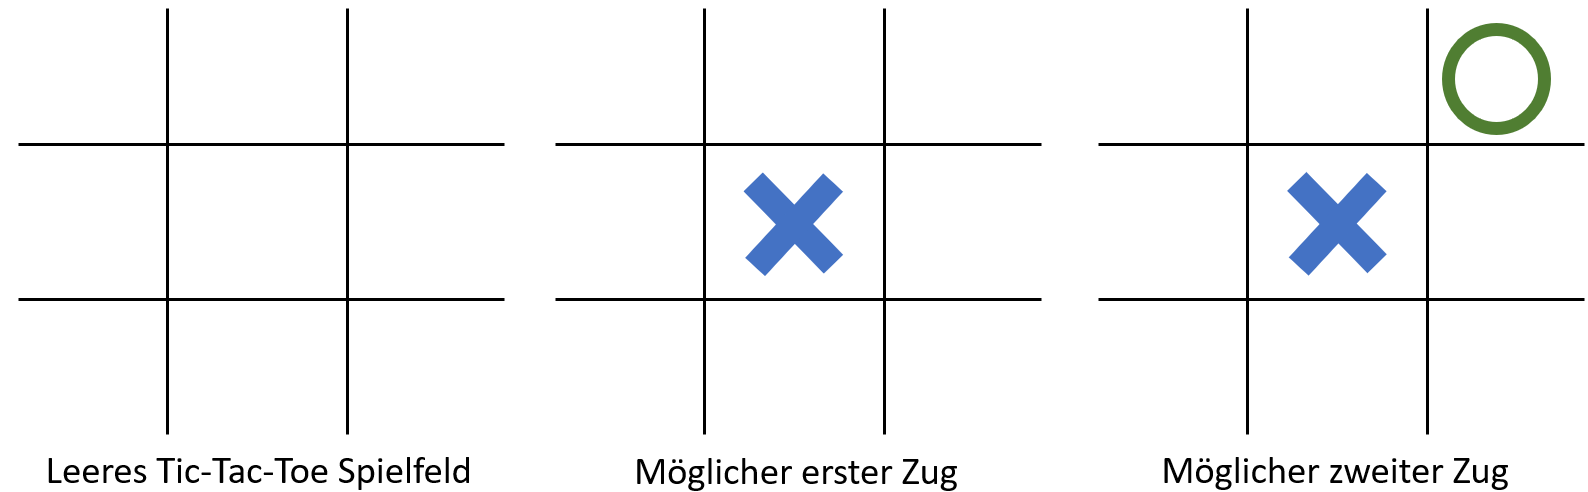
\includegraphics[scale=0.25]{img/tictactoe_start.png}
    \caption[Möglicher Anfang eines Tic-Tac-Toe Spiels]{Möglicher Anfang eines Tic-Tac-Toe Spiels (eigene Anfertigung)}
\end{figure}
Im ersten Teil des Bildes erkennt man die neun leeren Felder des Spielfeldes. Im zweiten Teil des Bildes fängt der erste
Spieler damit an, sein erstes Kreuz in die Mitte des Spielfeldes zu setzen. Der zweite Spieler ist nun am Zug und setzt
im dritten Teil des Bildes seinen Kreis in die obere rechte Ecke des Spielfeldes. Als nächstes wäre Spieler eins wieder an
der Reihe und dürfte sein nächstes Kreuz setzen. Ziel des Spiels ist es, drei gleiche Symbole in einer Reihe, Spalte oder
Diagonale zu haben. Die folgende Abbildung soll dieses Verfahren nochmal genauer erläutern:
\begin{figure}[H]
    \centering
    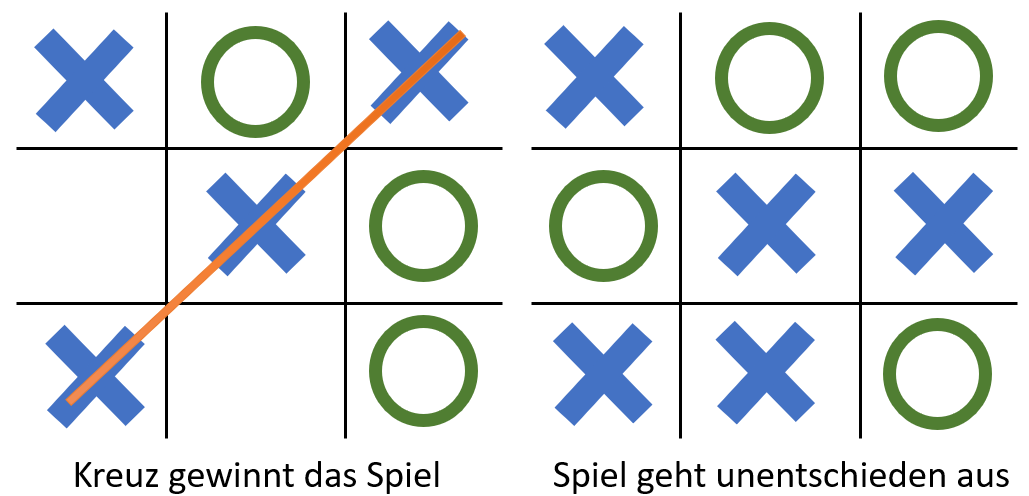
\includegraphics[scale=0.25]{img/tictactoe_endings.png} 
    \caption[Mögliches Ende eines Tic-Tac-Toe Spiels]{Mögliches Ende eines Tic-Tac-Toe Spiels (eigene Anfertigung)}
\end{figure}
Im ersten Teil der Abbildung ist zu sehen, wie der Spieler mit dem Kreuzsymbol drei Kreuze auf einer Diagonale unterbringen
konnte. In diesem Fall ist die Runde beendet und dieser Spieler hat die Runde gewonnen. Ob das Spiel über drei Symbole in einer
Reihe, Spalte oder Diagonale gewonnen wird, ist nicht relevant. Ebenfalls spielt es keine Rolle, in welcher Reihenfolge die 
Symbole gesetzt wurden. Im zweiten Teil des Bildes zeigt sich ein weiteres mögliches Ende für eine Runde Tic-Tac-Toe. Bei diesem
Ende ist das komplette Spielfeld ausgefüllt und es ergeben sich keine drei Symbole in einer Reihe, Spalte oder Diagonale. 
Entsprechend ist die Runde unentschieden ausgegangen.

\section{Der Minimax-Algorithmus}
Nachdem das Spiel Tic-Tac-Toe erklärt wurde, soll nun mit Hilfe des Minimax Algorithmus eine künstliche Intelligenz 
entwickelt werden, die in einem Spiel gegen einen menschlichen Spieler immer einen optimalen Zug ausführt. Der Minimax 
Algorithmus baut dabei auf der Funktion \code{value} auf, die wie folgt definiert ist:

\[value: States \times Players \rightarrow \{-1,0,1\}\]

Die Rückgabewert symbolisieren dabei den bestmöglichen Ausgang eines Zuges:

\begin{itemize}
    \item -1 bedeutet, dass der Spieler keine Möglichkeit mehr hat eine Niederlage zu verhindern
    \item 0 bedeutet, dass im besten Fall ein Unentschieden erzielt werden kann
    \item 1 bedeutet, dass ein Sieg möglich ist
\end{itemize}

Die Funktion bekommt also einen Zustand des Spielbretts und den Spieler für den der Wert berechnet werden soll.
Um den Rückgabewert zu berechnen, werden sämtliche mögliche Spielverläufe berechnet und 

\chapter{Praxis}

\section{Implementierung von Tic-Tac-Toe und Minimax}
Ziel dieses Kapitels ist es die Implementierung in Java zu erläutern. Da der Fokus dieser Arbeit jedoch auf der Performance
des Algorithmus in Java liegt und eine detaillierte Erläutertung der Implementierung sehr aufwendig wäre, folgt lediglich
ein grober Überblick über die meisten Aspekte der Implementierung. Lediglich Teile der Implementierung, die besonders relevant
für die Performance des Programms sind werden detaillierter erläutert. 

\subsection{Objektorientierung: Unterteilung in Klassen}
Zunächst folgt eine grobe Erläuterung der drei Klassen, in die die Implementierung unterteilt wurde.
Diese Klassen sind auch im folgenden Klassendiagramm zu sehen:
\begin{figure}[H]
    \centering
    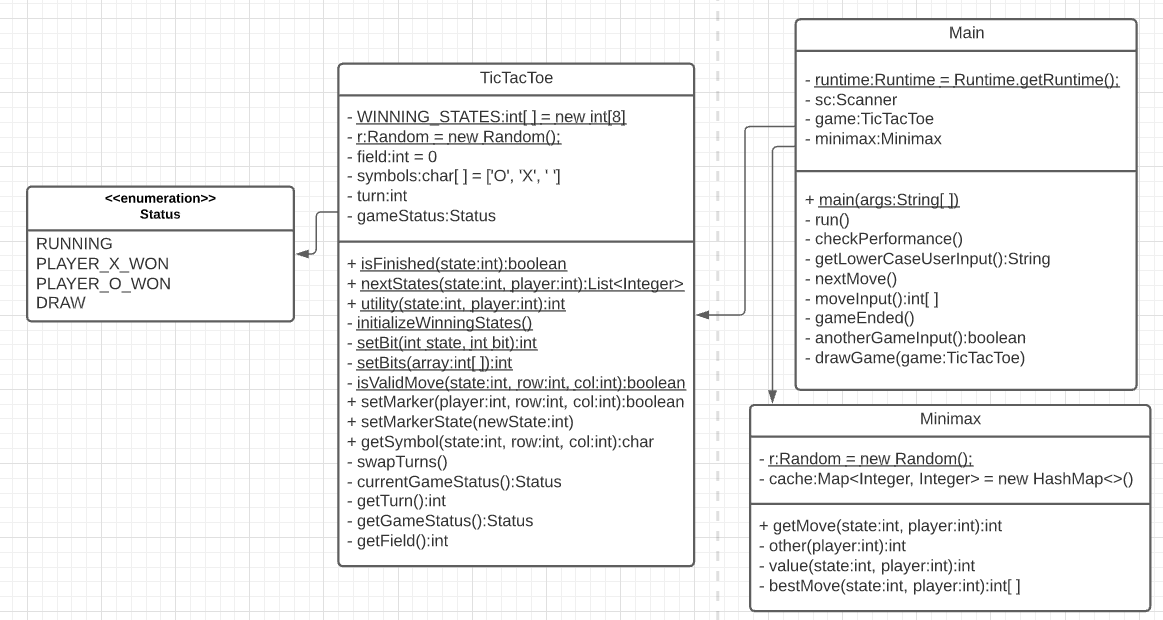
\includegraphics[scale=0.2]{img/uml_diagram.png}
    \caption[Vollständiges Klassendiagramm der Implementierung]{Vollständiges Klassendiagramm der Implementierung (eigene Anfertigung)} % TODO besseres Bild, sobald es richtig ist
    \label{fig:uml}
\end{figure}

\textbf{Main.java:} Diese Klasse enthält die main-Methode und ist der Startpunkt für das Programm. Sie ist sie dafür
verantwortlich, dass Objekte der anderen beiden Klassen erstellt und verwaltet werden. Die gesamte Logik, welche es ermöglicht, dass 
eine Person eine Runde Tic-Tac-Toe gegen den Minimax-Algorithmus spielen kann, ist in dieser Klasse. Hierzu gehören beispielsweise 
das Abfragen des nächsten Zuges der Person und des Algorithmus sowie alle Ein- und Ausgaben, die zur Bedienung des Programmes notwendig sind. 
Außerdem enthält diese Klasse die Funktion zur Messung der Performance, welche in Kapitel \ref{chap:performancevergleich} zum Einsatz kommt.

\textbf{TicTacToe.java:} Die Klasse TicTacToe ist, wie der Name schon sagt, die Klasse, in der die gesamte benötigte Logik für eine Runde
Tic-Tac-Toe enthalten ist. In dieser Klasse sind sowohl die möglichen Zustände, bei denen ein Spieler das Spiel gewonnen hat als auch der
aktuelle Zustand des Spielbretts gespeichert. Ebenfalls wird der Status des Spiels (siehe enum in Abbildung \ref{fig:uml}), sowie der Spieler, der aktuell
am Zug ist, gespeichert. Des Weiteren sind alle Funktionen enthalten, die zum Anzeigen oder Verändern des Spielfeldes benötigt werden. Hierzu
gehört auch eine Funktion, die ermittelt, ob der gegebene Zug zulässig ist oder das gewünschte Feld bereits belegt ist.

\textbf{Minimax.java:} Innerhalb der Klasse Minimax ist die gesamte Logik für den Minimax Algorithmus enthalten. Hierzu gehören alle Funktionen,
welche benötigt werden, um den bestmöglichen Spielzug bei einem bestimmten Spielstand zu ermitteln. Um alle notwendigen Parameter zu erhalten,
die für die Ermittlung des nächsten Spielzuges benötigt werden, ruft die Klasse Minimax teilweise statische Funktionen der Klasse TicTacToe auf,
welche die notwendigen Werte zurückliefern. Die relevanteste Funktion in dieser Klasse ist die rekursive Funktion \code{value(int state, int player)}, 
da diese in Kapitel \ref{chap:performancevergleich} zur Messung der Performance aufgerufen wird. Die Funktion dient der Bewertung eines möglichen 
Spielzustands anhand der möglichen Gewinnmöglichkeiten (siehe auch Kapitel \ref{chap:Minimax}).

\subsection{Performancerelevante Implementierungen im Detail}
\label{chap:implementierungen}
\subsubsection{Spielstand als Bitmaske}

\subsubsection{Caching von Folgezuständen}

\section{Performancevergleich von Java und Python}
\label{chap:performancevergleich}

Nachdem der Minimax-Algorithmus für das Spiel Tic-Tac-Toe in Java implementiert wurde, soll nun die 
Performance mit der Umsetzung in Python verglichen werden. Hierfür wird bei beiden Versionen die Funktion 
\code{value} für ein leeres Spielfeld mit Spieler 0 aufgerufen. D. h. die Funktion \code{value} berechnet 
alle möglichen Spielzustände und deren Wert. Die CPU-Zeiten beziehen sich auf eine Testreihe mit einem 
Intel i7-9700K. Für jeden Test werden jeweils fünf Durchgänge mit und ohne Memoisierung durchgeführt 
und daraus der Durchschnittswert berechnet.

\begin{table}[H]
    \centering
    \begin{tabular}{|l|ll|l|}
        \hline
        \multicolumn{4}{|l|}{\textbf{RAM}}                                             \\ \hline
                                & ohne memoize & mit memoize &                         \\ \hline
        \multirow{1}{*}{Python} &              & 808         & \multirow{7}{*}{in KB}  \\ \cline{1-3}
        \multirow{5}{*}{Java}   & 12875        & 1515        &                         \\
                                & 13392        & 1515        &                         \\
                                & 13387        & 1515        &                         \\
                                & 12881        & 1515        &                         \\
                                & 13391        & 1514        &                         \\ \cline{1-3}
        average                 & 13185,2      & 1514,8      &                         \\ \hline
    \end{tabular}
    \caption{Ergebnisse der Performancetestreihe für den genutzten Arbeitsspeicher}
\end{table}

Da für den belegten Arbeitsspeicher der Python Implementierung keine verlässlichen Messwerte gemessen werden 
konnten, wird der Messwert aus dem Jupyter-Notebook (Bitboard mit Memoisierung) verwendet. Auffallend ist, 
dass die Java Implementierung selbst mit Memoisierung, fast doppelt so viel Speicher verbraucht wird. 
Darüber hinaus kann durch Memoisierung bei der Implementierung in Java der Speicherverbrauch um den 
Faktor 8,5 reduziert werden.

\begin{table}[H]
    \centering
    \begin{tabular}{|l|ll|l|}
        \hline
        \multicolumn{4}{|l|}{\textbf{CPU Time}}                                        \\ \hline
                                & ohne memoize & mit memoize &                         \\ \hline
        \multirow{5}{*}{Python} & 2520         & 42,6        & \multirow{12}{*}{in ms} \\
                                & 2520         & 45          &                         \\
                                & 2520         & 44          &                         \\
                                & 2510         & 42          &                         \\
                                & 2510         & 44          &                         \\ \cline{1-3}
        average                 & 2516         & 43,92       &                         \\ \cline{1-3}
        \multirow{5}{*}{Java}   & 43           & 8           &                         \\
                                & 43           & 8           &                         \\
                                & 44           & 9           &                         \\
                                & 45           & 7           &                         \\
                                & 42           & 8           &                         \\ \cline{1-3}
        average                 & 43,4         & 8           &                         \\ \hline
    \end{tabular}
    \caption{Ergebnisse der Performancetestreihe für die benötigte Zeit}
\end{table}

Die Schnelligkeit der Python-Implementierung mit Memoisierung ist in etwa gleich zur Java-Implementierung 
ohne Memoisierung. Mit Memoisierung kann die Laufzeit durch die Verwendung von Java nochmal um 80\% verringert 
werden.

\section{Java vs. Python}
Neben den in Kapitel \ref{chap:implementierungen} gezeigten Unterschieden bei der Implementierung, können die in Kapitel 
\ref{chap:performancevergleich} ermittelten Performanceunterschiede durch Unterschiede in der Funktionsweise der 
Sprachen erklärt werden.

\subsection{Memory Management}
Während Python oft als unperformant wahrgenommen wird, konnte Python beim Arbeitsspeicherverbrauch im Vergleich 
zu Java punkten. Dies kann vorallem durch Unterschiede beim Speichermanagement der beiden Sprachen erklärt werden. 

Arbeitsspeicher wird in Python über einen Heap, der intern verwaltet wird. Wird also Arbeitsspeicher benötigt, 
wird dieser durch das Memory-Management vom Betriebssystem angefordert. Objekte bleiben nur so lange im Speicher 
wie sie benötigt werden. Python nutzt das sogenannte Reference Counting um Objekte zu speichern.

\begin{lstlisting}[caption={Codebeispiel zur Verwaltung von Objekten in Python}]
    a = 9
    b = 9
    c = 11
\end{lstlisting}

In diesem Beispiel wird der Wert 9 als Objekt im Speicher erstellt und Variable \code{a} zugewiesen. Da 
Das Objekt mit dem Wert 9 schon existiert, wir Variable {b} als weitere Referenz hinzugefügt. Für Variabl 
\code{c} heißt das, dass ein Objekt mit dem Wert 11 angelegt werden muss und \code{c} als Referenz hinterlegt wird. 
Beträgt die Anzahl der Referenzen eines Objekts Null, so wird es aus den Speicher entfernt. Die Referenzen 
werden zyklisch vom Garbage Collector überprüft und Objekte ohne Referenzen entfernt. Reference Counting 
hat den Vorteil, dass nicht genutzter Speicher sehr schnell erkannt wird. Allerdings entsteht durch das Zählen 
der Referenzen ein gewisser Overhead, der im Vergleich zu anderen Garbage Collecting Verfahren aber eher gering ausfällt.

%TODO: Garbage Collection Java
\chapter{Fazit \& Ausblick}

\section{Fazit}

\section{Ausblick}
Kleine Liste was vorkommen könnte (kannst aber selbstverständlich auch selbst irgendwas finden :D) 

- Speicherung in 1x Byte und 1x Short (8 Bit aus dem Byte und 16 Bit aus dem Short), um ein weiteres Byte zu sparen (int hat 4 byte). Evtl. auch
Speicherung mit 18 Booleans, aber ka ob das schneller ist. Als These könntest dus aber bringen

- Weitere Optimierung (auch in Einleitung angedeutet): Weiteres Caching (z. B. die NextStates und nicht nur deren Wert), Wechsel der Programmiersprache, Upgrade der CPU - 
oder sogar einmalige Speicherung des optimalen Zuges bei jedem Zustand, sodass dieser künftig direkt ausgewählt werden kann und der Algorithmus nur einmalig
durchlaufen werden muss, um alle Werte zu errechnen und zu Speichern

%	Literaturverzeichnis
\clearpage
\ihead{\chaptername~\thechapter} 
\ohead{\headmark} 
\pagenumbering{Roman}
\setcounter{page}{9}

\printbibliography[title=Literaturverzeichnis]

\cleardoublepage

%	Glossar
%\addcontentsline{toc}{chapter}{Glossar}
%% !TEX root =  master.tex
\chapter*{Glossar}



%\newpage

% Der Anhang beginnt hier - jedes Kapitel wird alphabetisch aufgezählt. (Anhang A, B usw.)
\appendix
\ihead{\appendixname~\thechapter} % Neue Header-Definition

%appendix.tex einziehen
\addcontentsline{toc}{chapter}{Anhang}
%% !TEX root =  master.tex

\end{document}